% Chapter 1

\chapter{Elliptic Curve Geometry} % Main chapter title

\label{EC} % For referencing the chapter elsewhere, use \ref{Chapter1} 

%----------------------------------------------------------------------------------------

% Define some commands to keep the formatting separated from the content 
\newcommand{\keyword}[1]{\textbf{#1}}
\newcommand{\tabhead}[1]{\textbf{#1}}
\newcommand{\code}[1]{\texttt{#1}}
\newcommand{\file}[1]{\texttt{\bfseries#1}}
\newcommand{\option}[1]{\texttt{\itshape#1}}

%----------------------------------------------------------------------------------------

\section{Introduction}
Bitcoin security is based on public and private key cryptograpy. The main concept is that it is simple to compute the public key, knowing the private, but it is infeasible to calculate the private key, knowing the public. \\ \\
In order to obtain this result a particular Elliptic Curve is used.

\section{Elliptic Curve over $\mathbb{F}_p$}

A point $Q$, which coordinates are $x$ and $y$, belong to an Elliptic Curve if and only if $Q$ satisfies the following equation:
\begin{equation}\label{GeneralEC}
y^2=x^3+ax+b \quad \textrm{over} \ \mathbb{F}_p
\end{equation}
Where $\mathbb{F}_p$ is the finite field defined over the set of integers modulo $p$ and $a$ and $b$ are the coefficients of the curve. \\ \\
We can rewrite the equation \ref{GeneralEC} in the following way:

\begin{equation}\label{GeneralECmodp}
y^2=x^3+ax+b \quad \textrm{mod} \ p
\end{equation}
Figure \ref{fig:EC_ex} shows some examples of Elliptic Curve over $\mathbb{F}_p$ with $a=-7$ and $b=10$
\begin{figure}[ht!]
	\centering
	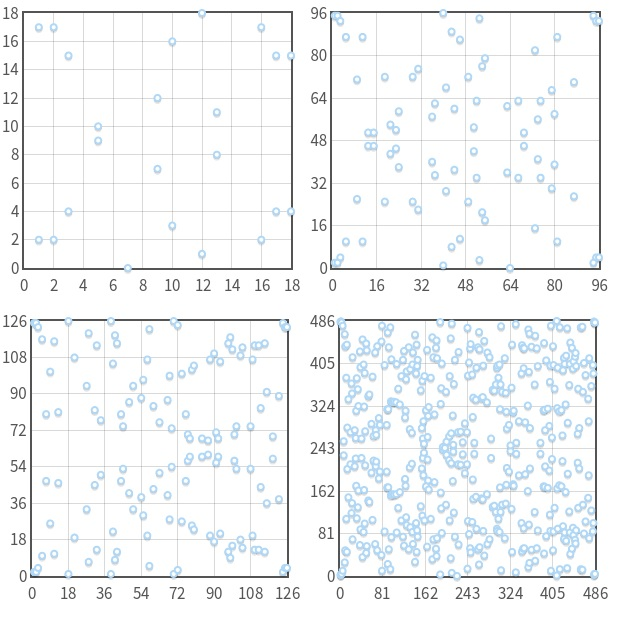
\includegraphics[width=9cm]{Figures/EC_ex.jpg}
	\caption{Points on the Elliptic Curve $y^2=x^3-7x+10 \; \textrm{mod} \ p$, with $p=19,97,127,487$ }
	\label{fig:EC_ex}
\end{figure}






\subsection{Operations}
A point on the Elliptic Curve has some particular properties:
\begin{itemize}
	\item Symmetry
	\item Point addition
	\item Scalar multiplication
\end{itemize}

\subsubsection{Symmetry}
For every point in the $x$ axis exists two points in the $y$ axis. Suppose that a point $P(x,y)$ belongs to the Elliptic Curve, then it must satisfy the equation \ref{GeneralEC}.
So it is easy to prove that the point $Q(x,p-y)$ belongs to the curve too. \\ \\
Furthermore we have $P=-Q$, from the moment that $P+Q=0$ (see addition below).

\subsubsection{Point addition}
We need to change our definition of addition in order to make it works in $\mathbb{F}_p$. 
In this framework we claim that if three points are aligned over the finite field $\mathbb{F}_p$, then they have zero sum. \\
So $P+Q=R$ if and only if $P$, $Q$ and $-R$ are aligned, in the sense\ shown in figure \ref{fig:EC_aligned}
\begin{figure}[ht!]
	\centering
	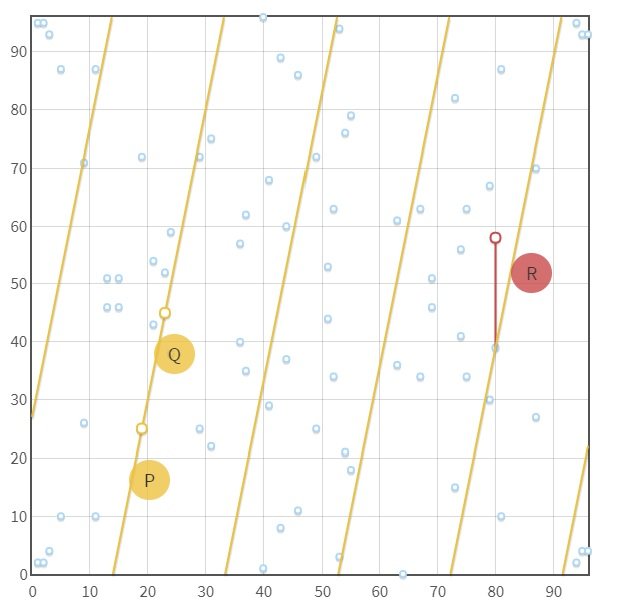
\includegraphics[width=9cm]{Figures/EC_aligned.jpg}
	\caption{Elliptic Curve $y^2=x^3-7x+10 \; \textrm{mod} \ 97$}
	\label{fig:EC_aligned}
\end{figure}


The equations for calculating point additions are the follow: \\
Suppose that \textit{A} and \textit{B} belong to the Elliptic Curve.

\begin{center}
	$ A=(x_1,y_1) \quad B=(x_2,y_2)$
\end{center}
Let's defined $ A+B :=(x_3,y_3) $ \\
So we have: 

\begin{center} 
	$s=\begin{cases} \dfrac{y_2-y_1}{x_2-x_1}, & \mbox{if } x_1\neq x_2 \\ \\ \dfrac{3x_1^2+a}{2y_1}, & \mbox{if } x_1= x_2\end{cases}$ 
\end{center}
\begin{center} 
	$ x_3=s^2-x_1-x_2  \quad$ mod $p$\\
	$y_3=s(x_1-x_3)-y_1  \quad$mod $p$
\end{center}

\subsubsection{Scalar multiplication}
Once defined the addition, any multiplication can be defined as:
\begin{center} 
	$ nP=\underbrace{
		P+P+\cdot \cdot \cdot+P
	}_{n\text{ times}}$
\end{center}
When $n$ is a very large number can be difficult or even infeasible to compute $nP$ in this way, but we can use the \textit{double and add algorithm} in order to perform multiplication in $\mathcal{O}(\log{}n)$ steps.

\subsection{Group order}
An elliptic curve defined over a finite field is a group and so it has a finite number of points. This number is called order of the group.\\
If the prime order is a very large number, it is impossible to count all the point in that field, but there is an algorithm that allows to calculate the order of a group in a fast and efficient way: \textit{Schoof's algorithm}.

\subsubsection{Cyclic subgroups}
Let's consider a generic point $P$, we have:
\begin{center} 
	$ nP+mP=\underbrace{
		P+\cdot \cdot \cdot+P
	}_{n\text{ times}}+
		\underbrace{
		P+\cdot \cdot \cdot+P
	}_{m\text{ times}}=
	\underbrace{
		P+\cdot \cdot \cdot+P
	}_{n+m\text{ times}} = 
	(n+m)P$
\end{center}
So multiple of $P$ are closed under addition and this is enough to prove that the set of the multiples of $P$ is a cyclic subgroup of the group formed by the elliptic curve.
\\ \\
The point $P$ is called \textbf{generator} of the cyclic subgroup.

\begin{remark}
	The order of $P$ is linked to the order of the elliptic curve by Lagrange's theorem, which states that the order of a subgroup is a divisor of the order of the parent group.
\end{remark}

\begin{remark}
	If the order of the group is a prime number, all the point $P$ generate a subgroup with the same order of the group.
\end{remark}



\section{Bitcoin private-public key cryptography}

\subsection{Bitcoin Elliptic Curve}
Bitcoin uses a specific Elliptic Curve defined over the finite field of the natural numbers, where $a=0$ and $b=7$. \\ \\
The equation \ref{GeneralEC} becomes:

\begin{equation}\label{BitcoinEC}
y^2=x^3+7 \quad \textrm{mod} \ p
\end{equation}

The \textit{mod p} (modulo prime number) indicates that this curve is over a finite field of prime order $p=2^{256}-2^{32}-2^9-2^8-2^7-2^6-2^4-1$.
\\ \\
The \textit{order} of this Elliptic Curve is a very large prime number, close to $2^{256}$, but smaller then $p$. \\ \\
Let's consider a particular point $G$, called generator, with:
\begin{center} 
	$ x=79BE667E F9DCBBAC 55A06295 CE870B07 029BFCDB 2DCE28D9 59F2815B 16F81798$\\
	$y=483ADA77 26A3C465 5DA4FBFC 0E1108A8 FD17B448 A6855419 9C47D08F FB10D4B8$
\end{center}

From the moment that the order of the group is a prime number, the order of any subgroup is equal to the order of the entire group. In particular the order of the subgroup generated by $G$ is equal to \textit{order}.

\begin{definition}
	A private key is a number choosen in the range beetwen 1 and \textbf{order}.
\end{definition}

\begin{definition}
	A public key $W$ is a point in the Bitcoin EC, derived from a private key $k$ in the following way: \\
	\begin{equation}
		W=k\cdot G
	\end{equation}
	Where the multiplication between k and G is defined in the previous chapter.
\end{definition}

This is a \textit{one way} function, in the sense that computing the scalar multiplication, knowing the private key is simple, but make the reverse is infeasible.
\begin{remark}
	It is infeasible to calculate a private key knowing the public key.
\end{remark}


\subsection{Bitcoin keys rapresentation and addresses}
In order to make it easy to store and recognise keys, some encods were designed.
\\ \\
A public key, a point in the EC, can be rapresented in two way: \textit{uncompressed} or \textit{compressed}.\\ \\
\subsubsection{Uncompressed public key}
An uncompressed public key is rapresented in hexadecimal digits, and it is obtained simply concatenating the $x$ coordinate with the $y$ coordinate and adding $04$ at the beginning, for a total of $130$ hexadecimal digits. \\ \\
Example of an uncompressed public key: \\
0450863AD64A87AE8A2FE83C1AF1A8403CB53F53E486D8511DAD8A04887E5B235 22CD470243453A299FA9E77237716103ABC11A1DF38855ED6F2EE187E9C582BA6


\subsubsection{Compressed public key}
A compressed public key is obtained simply taking the $x$ coordinate and adding $02$ at the begging if the $y$ coordinate is even, $03$ otherwise. \\
This is due to the \textit{symmetry properties} of a point of the EC.
\\ \\
Example of a public key compressed:\\
0250863AD64A87AE8A2FE83C1AF1A8403CB53F53E486D8511DAD8A04887E5B2352


\subsubsection{WIF Private Key}
WIF stands for wallet import format and is the standard way used to write down a private key.
\begin{itemize}
	\item Add a version number ($80$ for Bitcoin) in front of the private key, in order to recognize quickly for what cryptocurrency that private key was used.
	\item Add $01$ at the end of the private key if you want a WIF \textit{compressed}, none if you want a WIF \textit{uncompressed}. The difference between these two types is that from a \textit{compressed} private key a \textit{compressed} public key is expected and from a \textit{uncompressed} private key a \textit{uncompressed} public key is expected.
	\item Addd a checksum at the end, obtained applying the SHA256 function twice to the string previously obtained, take the first 4 bytes (8 hexadecimal digits) and put them at the end of the string.
	\item Compute the Base58Encode, obtaining a 52 digit string.
\end{itemize}
Example of private key WIF: \\ KwdMAjGmerYanjeui5SHS7JkmpZvVipYvB2LJGU1ZxJwYvP98617

\subsubsection{Address}
Among the Bitcoin transactions, one of the most used is a \textit{Pay-to-PubkeyHash}, meaning that in the transaction you will not write directly the public key, but the hash of that public key.
\\
The hash function used in this freamwork is the HASH160 function, applied to the \textit{compressed} public key. This is an irreversible procedure, so you cannot obtain the public key from the public key hash. \\ \\
In order to obtain a valid Bitcoin address, it is needed to encode the \textit{PubkeyHash} in base58, adding first the version in front, the checksum at the end and then encode everything with Base58Encode, obtaining a 34 digit string. 
\\ \\
Example of an Address: \\
1BvBMSEYstWetqTFn5Au4m4GFg7xJaNVN2



